\chapter{3D-Echtzeitrendering in Unity}
\label{ch:3drender}
3D-Rendering bezeichnet den Prozess, bei dem der Inhalt einer dreidimensionalen, virtuellen Szene, in ein zweidimensionales Bild umgewandelt wird. Ähnlich, wie bei der Aufnahme einer Filmszene muss hier die Szene vorbereitet, die Kamera positioniert und die Beleuchtung entsprechend der gewünschten Ansicht ausgerichtet werden. Der große Unterschied bei 3D-Rendering im Vergleich zu Realfilmaufnahmen besteht darin, dass alle Bestandteile der Szene zunächst von 3D-Artists erstellt werden müssen. Das schließt die Modellierung und Texturierung der Modelle sowie das \name{shading} der Oberflächen ein (vgl. \cite{Neumann.11.11.2020}). Zusätzlich können die fertigen 3D-Modelle noch animiert werden. Zum Schluss muss der Szene noch eine passende Beleuchtung hinzugefügt werden. Erst nach Abschluss dieser Arbeitsschritte kann mit Hilfe einer virtuellen Kamera eine fertige 3D-Szene gerendert werden. Abhängig vom verwendeten Render-Algorithmus kann die Berechnung eines einzigen Bildes vom Bruchteil einer Sekunde bis hin zu mehreren Tagen in Anspruch nehmen. \name{rasterization} und \name{raytracing} \ref{sec:rzvsrt} sind dafür die am häufigsten eingesetzten Techniken (vgl. \cite{Emiliano.08.08.2019}).
%
	\section{Bestandteile einer 3D-Szene}
	\label{sec:3dsetup}
	Um eine virtuelle Szene zu rendern, sind neben der virtuellen Kamera und netzbasierten Objekten eine Reihe grundlegender Ressourcen erforderlich. In diesem Abschnitt werden lediglich die vier essentiellen Bestandteile einer 3D-Szene erläutert. Alle weiteren Elemente, wie z.B. Partikelsysteme oder \name{post-processing-effects}, waren für die Entwicklung und Visualisierung der \mapp des \vmds nicht erforderlich. Die Basis einer virtuellen 3D-Szene bilden die \name{3D-Meshes}, im Folgenden als \name{meshs} bezeichnet. Polygone \gerref{Vielecke}, sind im \name{Rendering}-Kontext gleichbedeutend mit Dreiecken. Sie sind die kleinste Flächeneinheit und bilden aneinander gereiht die Oberflächen der 3D-Objekte. Die Polygone können außerdem in ihre \name{faces} \gerref{Flächen}, \name{edges} \gerref{Kanten} und \name{vertices} \gerref{Punkte} unterteilt werden \figref{\ref{fig:polyhedra-edge-face-vertex}}. Um die 3D-Modelle in der Szene farbig darstellen zu können, sind Texturen erforderlich. Es handelt sich dabei meist um Bilddateien, die anhand von \name{UV-maps} bzw. Texturkarten eines 3D-Models auf diesem dargestellt werden können. Eine \name{UV-map} ist die zweidimensionale Darstellung, eines 3D-Modells. Diese wird erstellt, indem ein Modell im \name{UV-mapping} auseinander geklappt wird \figref{\ref{fig:uv_map}}. Dieser Schritt ist erforderlich, da ein 3D-Modell ausschließlich im dreidimensionalen Raum existiert. Die Nutzung von Bild-Texturen setzt allerdings eine Konvertierung des Modells in den zweidimensionalen Raum voraus. Die Texturen können auch verschiedene Eigenschaften zugewiesen bekommen, die dann miteinander kombiniert in den \enquote{Textur-Kanälen} eines \name{materials} Verwendung finden. An dieser Stelle werden lediglich die drei \enquote{Textur-Kanäle} erläutert, die zur Darstellung der 3D-Modelle in der \mapp verwendet wurden. Für die Einfärbung der Oberfläche ist der \name{albedo}-Kanal bzw. die \name{albedo}-Textur verantwortlich. Dabei handelt es sich um eine Texturkarte, deren Pixelwerte als Farbwerte interpretiert werden. Sollte innerhalb einer Textur Transparenz zum Einsatz kommen, wird diese Information in Unity ebenfalls in der \name{albedo}-Textur hinterlegt. Die \name{metallic}-Textur bekommt ein schwarz-weiß Bild zugewiesen, das anschließend als Maske interpretiert wird, um metallische von nicht-metallischen Oberflächen unterscheiden zu können. Diese Textur ist primär für die Reflexionseigenschaften der virtuellen Oberfläche verantwortlich. Die Aufgabe der \name{normal map} besteht darin, Oberflächendetails innerhalb der Textur darzustellen, auch wenn diese im \name{mesh} des 3D-Modells nicht vorhanden sind. Eine \name{normal map} speichert die Ausrichtungen der Normalenvektoren einer Oberfläche in Form von Farbcodierungen als Textur und ermöglicht die Darstellung von Details, ohne dass diese im \name{mesh} vorhanden sind. Dieser letzte Schritt ist besonders wichtig für den sogenannten \enquote{high-poly to low-poly workflow} (vgl. \cite{Neumann.11.11.2020}). Sofern das Licht der virtuellen Szene mit den Oberflächen der 3D-Modelle und den Eigenschaften der \name{materials} interagieren soll, ist der Einsatz von \name{shadern} erforderlich. Das sind Programme, die in erster Linie mathematische Berechnungen mit verschiedenen Algorithmen ausführen. Ein \name{shader} hat die Aufgabe, aus den Beleuchtungswerten der Szene und den \name{material}-Eigenschaften einer Oberfläche den korrekten Farbwert eines Pixels auf dem Monitor zu ermitteln. Er bestimmt auch maßgeblich den Grafikstil, in dem die 3D-Szene gerendert wird (vgl. \cite{res.14.01.2021}). Im Rahmen der \mapp sollten realistische Modelle und damit kein spezieller künstlerischer Stil dargestellt werden. Unitys \name{standard-shader} ist bereits für das Rendern realistischer Szenen  mit dem \name{rasterization}-Algorithmus voreingestellt. Deshalb waren an dieser Stelle keine weiteren Anpassungen erforderlich.
	%
	\begin{figure}
		\centering
		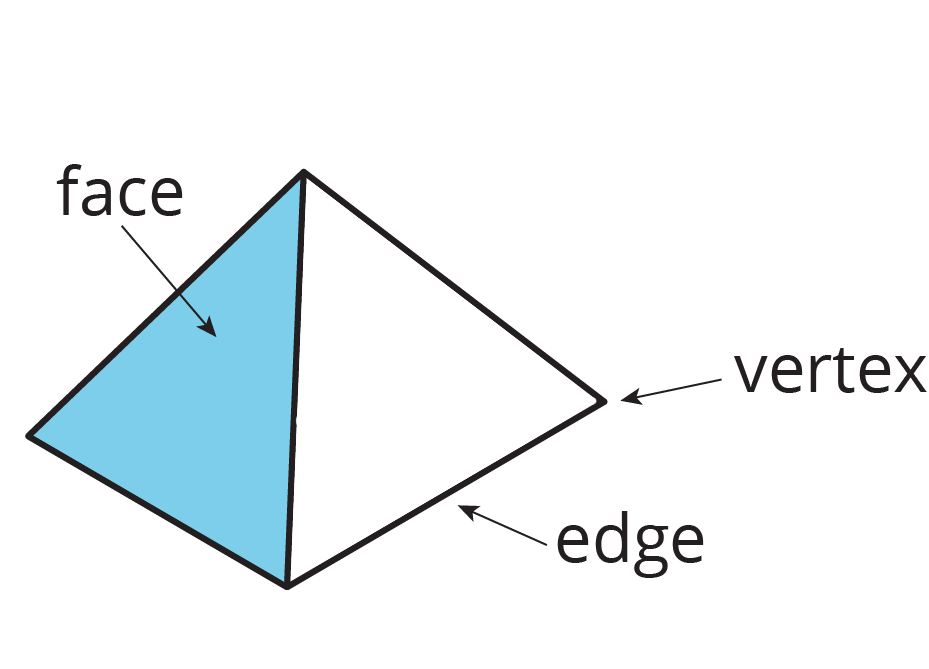
\includegraphics[width=0.6\linewidth]{images/polyhedra-edge-face-vertex}
		\captionsetup{justification=raggedright,singlelinecheck=false} %caption linksbündig
		\caption[polygon]{\\Unterteilung eines \name{Polygons} in \name{face}, \name{edges} und \name{vertices} \cite{oml.14.05.2020}}
		\label{fig:polyhedra-edge-face-vertex}
	\end{figure}
	%
	\begin{figure}
		\centering
		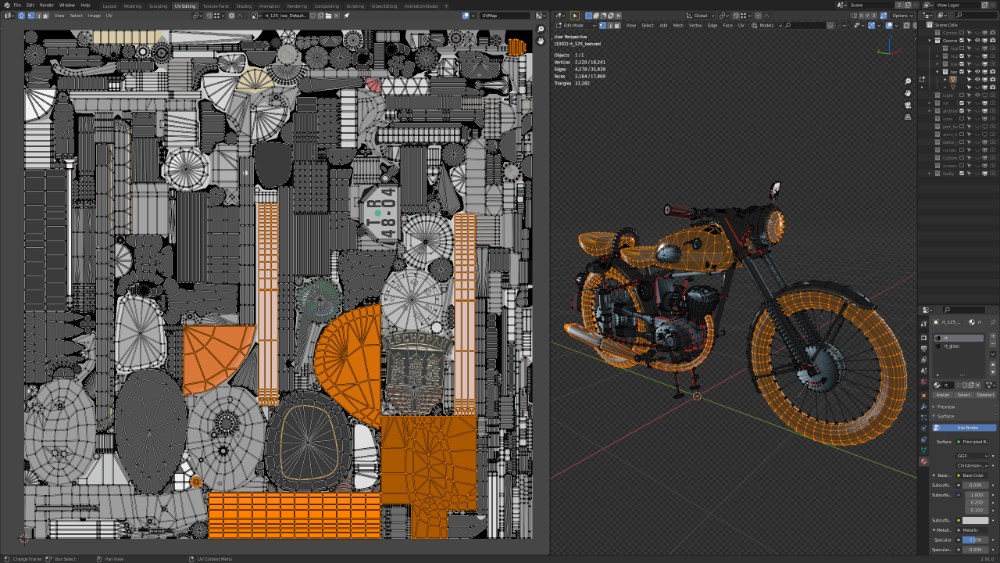
\includegraphics[width=0.9\linewidth]{images/uv_map}
		\caption[uv_map]{\\Die UV-Map der \name{MZ RT125} links und das vollständige Modell inklusive Texturen rechts}
		\label{fig:uv_map}
	\end{figure}
	%
	\section{Rasterization im Vergleich zu Raytracing}
	\label{sec:rzvsrt}
	Die Render-Algorithmen lassen sich in zwei Kategorien unterteilen: Online- bzw. Echtzeitrendering und Offline-Rendering. \name{Rasterization} zählt in die Kategorie des Echtzeitrendering und kommt beispielsweise bei der Erstellung von Videospielen oder für interaktive Benutzeroberflächen zum Einsatz. Um interaktive Systeme auf Basis von 3D-Rendering zu ermöglichen, ist eine hohe Bildwiederholrate erforderlich. Diese wird meistens in \acs{FPS} angegeben und steht für \name{frame per second} \gerref{Bilder pro Sekunde}. Die Bildwiederholrate sollte dabei mindestens 30 \acs{FPS} betragen, damit das menschliche Auge keine Einzelbilder mehr wahrnimmt, sondern einen flüssigen Bewegungsablauf (vgl. \cite{Teo.15.10.2010}). Videospiele zielen deshalb auf 30, 60 oder höhere \acs{FPS}-Werte ab, um den Fokus des Nutzers vollständig auf die virtuellen Interaktionen zu lenken (vgl. \cite[S.1]{AkenineMoller.2018}). Um diese hohe Bildwiederholrate zu gewährleisten, wird bei \name{rasterization} keine physikalisch korrekte Lichtberechnung durchgeführt, sondern es werden lediglich die 3D-Modelle auf das Raster der Monitorpixel projiziert. Durch diese Form der Kalkulation ist \name{rasterization} beispielsweise nicht in der Lage, Schatten und Reflexionen physikalisch korrekt darzustellen. Offline-Rendering bezeichnet das Verfahren, das meistens für Animationsfilme zum Einsatz kommt. Hier spielt die Rechengeschwindigkeit eine untergeordnete Rolle. Stattdessen liegt der Fokus auf physikalisch korrekter Lichtsimulation und der Qualität des Ergebnisses. Um dieses Ziel zu erreichen, kommen \name{raytracing}-Algorithmen zum Einsatz. Auf diese Weise können fotorealistische Schatten, Reflexionen und Lichtbrechungen physikalisch korrekt dargestellt werden \cite{Whitted.1980}. Diese Methode wird allerdings in den meisten Fällen für vorab gerenderte Bilder oder Videosequenzen eingesetzt, da hier die Berechnung eines Bildes, je nach verfügbarer Rechenleistung und Komplexität der Szene, oft mehrere Stunden oder auch Tage dauern kann. Da die Zielgeräte nur über relativ schwache Grafikchips verfügen und in der Zielstellung festgelegt wurde, dass die \mapp des \vmds direkte Interaktionen mit den virtuellen Fahrzeugmodellen ermöglichen soll, kommt für diesen Anwendungsfall ausschließlich die \name{rasterization}-Technik in Frage.
	%
	\newpage
	%	
	\section{Umsetzung als Render-Pipeline}
	\label{sec:RP}
	Eine Render-Pipeline hat die Aufgabe, auf Basis von Eingabe-Ressourcen eine Reihe von Berechnungen durchzuführen und anschließend das Ergebnis der Berechnungen auf dem Monitor darzustellen. Im Fall von Echtzeit-3D-Rendering sind 3D-Modelle mit ihren zugehörigen Texturen und \name{shadern} die Eingabe-Ressourcen. Das Ziel besteht darin, das \name{render-target} zu berechnen. Im 3D-Rendering ist das \name{render-target} die Projektion eines 3D-Modells auf die Pixel des Monitors. Um dieses Ergebnis zu ermitteln, setzt sich eine \name{rasterization}-Render Pipeline (kurz: \acs{RP}) aus vier Arbeitsschritten zusammen: \name{input assembler}, \name{geometry processing}, \name{rasterization} und \name{pixel processing} \figref{\ref{fig:rasterizationpipeline}}. Jeder dieser Schritte ist erneut in mehrere untergeordnete Arbeitsschritte unterteilt. Diese Zerlegung in viele kleine Schritte erlaubt die parallele Verarbeitung dieser Berechnungen. Die Schritte der Pipeline lassen sich in \name{fixed function stages} und programmierbare \name{shader} unterteilen. Erstere sind bis auf einzelne Parameter nur geringfügig steuerbar, während alle \name{shader} vollständig programmierbar und damit anpassbar sind. Zu Beginn liegen die 3D-Modelle lediglich als Punkt-Koordinaten im Speicher vor und müssen von der Render-Pipeline \enquote{zusammengebaut} \engref{assembled} werden. Deshalb wird die erste Phase der Pipeline \enquote{Input-Assembler} genannt. Dieser erste Arbeitsschritt wird von der jeweiligen Anwendung für gewöhnlich über den Prozessor (kurz: \acs{CPU}) initialisiert. An dieser Stelle werden die erforderlichen Daten aus dem Speicher geladen. Bei einer 3D-Szene bestehen die Daten hauptsächlich aus \name{vertices} (3D-Punkte) und Texturen (meistens Bilddateien). Zudem starten alle weiteren Berechnungen, die vor der Kalkulation eines neuen Frames ausgeführt werden müssen. Dazu zählen u.a. Kollisions-Abfragen, Animationen, Physik-Simulationen usw. Im nächsten Schritt, dem \name{geometry processing}, können alle geladenen \name{vertices} transformiert werden. Hier wird festgelegt, was im nächsten, zu berechnenden Frame auf dem Bildschirm dargestellt wird und wo es sich, bezogen auf die Position der Pixel, befinden soll. Dieser Schritt wird in den meisten Fällen bereits auf dem Grafikprozessor \engref{Graphics Processing Unit} (kurz: \acs{GPU}) ausgeführt, da ab diesem Pipeline-Schritt die Berechnungen i.d.R. parallel abgearbeitet werden können. Eine \acs{GPU} verfügt im Gegensatz zu einer \acs{CPU} oft über tausende programmierbare Rechenkerne, die auf Parallelverarbeitung ausgelegt sind. Somit kann der Grafikchip alle parallelen Berechnungen deutlich schneller ausführen als eine \acs{CPU}. Im nächsten Schritt folgt die namensgebende Rasterung \engref{rasterization}. An dieser Stelle werden jeweils drei \name{vertices} eines 3D-Modells, die ein zusammenhängendes Dreieck \engref{triangle} bilden, herausgenommen und alle Pixel ermittelt, die sich innerhalb dieses Bereichs befinden \figref{\ref{fig:rasterization}}. Dieser Vorgang wird für alle \name{vertices} der 3D-Objekte ausgeführt, die sich im Kamerasichtfeld befinden. Schließlich folgt das \name{pixel processing}. In diesem letzten Arbeitsschritt wird für jeden Pixel ermittelt, welche Farbe er erhalten soll und zusätzlich bestimmt der \name{Z-buffer}, ob der berechnete Pixel sichtbar oder verdeckt ist. Der \name{Z-buffer} speichert die Entfernung von Objekten zur Kamera. Durch diesen Wert können Aussagen über Sichtbarkeit der berechneten Pixel getroffen werden \cite{Catmull.1998}. Dieses Vorgehen ermöglicht beispielsweise das Übereinanderblenden verschiedener Farben zur Darstellung von transparenten Oberflächen. Die Arbeitsschritte \name{rasterization} und \name{pixel processing} setzen sich aus vielen Einzelschritten zusammen und werden i.d.R. vollständig auf der \acs{GPU} ausgeführt, um eine effiziente Parallelverarbeitung der einzelnen Phasen sicherzustellen \cite[S.13]{AkenineMoller.2018}. Allerdings würde das direkte Ansteuern der Hardware bzw. des Grafikchips für jeden Entwickler einen sehr hohen Programmieraufwand mit sich bringen. Aus diesem Grund wurden Programmierschnittstellen entworfen, die das Ansteuern des Grafikchips erleichtern. Die beiden bekanntesten Schnittstellen sind \name{DirectX} von Microsoft und \name{OpenGL} von der \name{Khronos Group}. Diese Schnittstellen bilden aber lediglich die Softwaregrundlage zur direkten Ansteuerung der Hardware. Wie genau die zahlreichen programmierbaren \name{Shader} dieser Pipeline implementiert werden, bleibt dabei den Entwicklern überlassen. Im folgenden Abschnitt werden die zwei Implementierungen der \name{Rasterization}-Pipeline innerhalb der Unity-Engine genauer betrachtet, die sich für die \mapp als relevant herausgestellt haben.
	%
	\begin{figure}
		\centering
		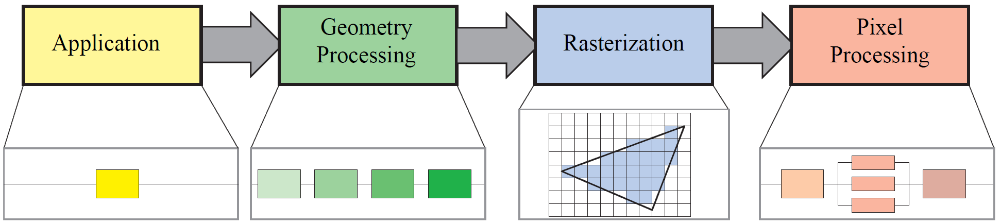
\includegraphics[width=0.8\linewidth]{images/rasterization_pipeline}
		\caption[ras_pipe]{\\Eine stark vereinfachte Darstellung der \name{rasterization}-Pipeline \cite[S.12]{AkenineMoller.2018}.}
		\label{fig:rasterizationpipeline}
	\end{figure}    
	%
	\begin{figure}
		\centering
		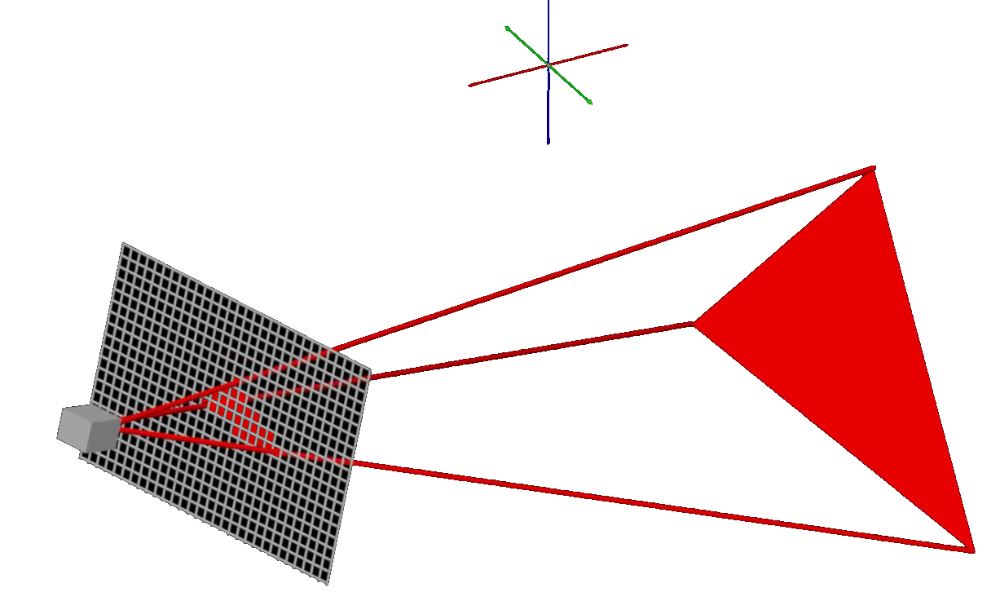
\includegraphics[width=0.6\linewidth]{images/rasterization}
		\caption[rasterization]{\\Das Dreiecks wird während der \name{rasterization}-Phase auf das Pixelraster des Monitors projiziert \cite{fm.15.01.2021}.}
		\label{fig:rasterization}
	\end{figure}
%